%  !TeX  root  =  user_guide.tex
% % \section{Working with Projections}\label{label_projections}
\chapter{Utiliser les projections}\label{label_projections}
% \index{Projections!working with}
\index{Projections!utiliser les}

% when the revision of a section has been finalized, 
% comment out the following line:
%\updatedisclaimer

% \qg allows users to define a global and project-wide CRS (Coordinate
% Reference System) for layers without a pre-defined CRS. It also allows the
% user to define custom coordinate reference systems and supports on-the-fly
% (OTF) projection of vector layers. All these features allow the user to
% display layers with different CRS and have them overlay properly.
\qg permet à l'utilisateur de définir un Système de Coordonnées de Référence  (SCR) par défaut ou pour l'ensemble d'un projet, pour les couches démunies de  SCR prédéfini. Il lui permet également de définir des systèmes de coordonnées  de référence personnalisés et autorise la projection à la volée de couches  vectorielles. Toutes ces fonctionnalités permettent à l'utilisateur d'afficher  des couches avec différents SCR et de les superposer correctement.

% \section{Overview of Projection Support}\label{label_projoverview}
\section{Aperçu de la gestion des projections}\label{label_projoverview}

% \qg has support for approximately 2,700 known CRS. Definitions for 
% each of these CRS are stored in a SQLite database that is installed with
% \qg. Normally you do not need to manipulate the database directly. In fact,
% doing so may cause projection support to fail. Custom CRS are stored in a
% user database. See Section \ref{sec:customprojections} for
% information on managing your custom coordinate reference systems.
\qg gère approximativement 2 700 SCR connus. Les définitions pour chacun d'entre eux sont stockées dans une base de données SQLite qui est installée avec \qg. Normalement vous n'avez pas besoin de manipuler cette  base de données directement. En fait, cela peut poser des problèmes de gestion de projections. Les SCR personnalisés y sont stockés dans une base de données utilisateur. Reportez-vous à la section \ref{sec:customprojections}  pour avoir des informations sur la gestion de vos systèmes de coordonnées de référence personnalisées.

% The CRS available in \qg are based on those defined by
% EPSG\index{EPSG} and are largely abstracted from the spatial\_references 
% table in PostGIS\index{PostGIS} version 1.x. The EPSG identifiers are
% present in the database and can be used to specify a CRS in \qg.
Les SCR disponibles dans \qg sont basés sur ceux définis par l'EPSG\index{EPSG} et sont en grande partie extraits de la table spatial\_references de PostGIS\index{PostGIS} (version 1.x). Les identifiants EPSG sont présents dans la base de données et peuvent être utilisés pour définir un SCR dans \qg. 

% In order to use OTF projection, your data must contain information about its
% coordinate reference system or you have to define a global, layer or
% project-wide CRS. For PostGIS layers \qg uses the spatial reference
% identifier that was specified when the layer was created. For data supported
% by OGR, \qg relies on the presence of a format specific means of specifying
% the CRS. In the case of shapefiles, this means a file containing the Well
% Known Text (WKT)\index{WKT} specification of the CRS. The projection file
% has the same base name as the shapefile and a prj extension. For example, a
% shapefile named \filename{alaska.shp} would have a corresponding projection
% file named \filename{alaska.prj}.
Dans le but d'utiliser la projection à la volée, vos données doivent contenir des informations sur leur système de coordonnées de référence sinon vous devrez définir un SCR global, par projet, ou bien par couche. Pour les couches PostGIS, \qg utilise l'identifiant de référence spatiale qui a été défini quand la couche a été créée. Pour les données gérées par OGR, \qg utilise un moyen spécifique au format pour définir le SCR. Dans le cas du shapefile, il s'agit d'un fichier contenant une spécification Well Known Text (WKT)\index{WKT} de la projection. Le fichier de projection a le même nom que le fichier shape et une extension prj. Par exemple, un shapefile nommé \filename{alaska.shp} aura un fichier de projection correspondant nommé \filename{alaska.prj}.

%Whenever you select a new CRS, the used layer units will automatically be 
%changed in the \tab{General} tab of the 
%\dropmenuopttwo{mActionOptions}{Project Properties} dialog under the 
%\mainmenuopt{Edit} (Gnome, OSX) or \mainmenuopt{Settings} (KDE, Windows) 
%menu.

Lorsque vous sélectionnez un nouveau SCR, les unités des couches utilisées seront automatiquement changées dans le panneau \tab{Général} de la fenêtre des \dropmenuopttwo{mActionOptions}{Propriétés du projet} du menu \mainmenuopt{Fichier} (Gnome, OSX) ou \mainmenuopt{Préférences} (KDE, Windows).

% \section{Specifying a Projection}
\section{Définir une projection}
% \index{Projections!specifying}
\index{Projections!définition}
\label{sec:projection-specifying}

% \qg no longer sets the map CRS to the coordinate reference system of the
% first layer loaded. When you start a \qg session with layers that do not
% have a CRS, you need to control and define the CRS definition for these
% layers. This can be done globally or project-wide in the \tab{CRS} tab under
% \mainmenuopt{Edit} > \dropmenuopttwo{mActionOptions}{Options} (Gnome, OSX) 
% or \mainmenuopt{Settings} > \dropmenuopttwo{mActionOptions}{Options} (KDE, Windows). 
% See Figure~\ref{fig:crsdialog}. 
\qg ne définit plus le système de coordonnées de référence à partir de  celui de la première couche chargée. Lorsque vous démarrez une session \qg avec des couches qui sont dépourvues de SCR, vous devez contrôler et définir le choix de la projection pour ces couches. Cela peut être réalisée globalement ou par projet dans l'onglet \tab{SCR} dans \mainmenuopt{Préférences} > \dropmenuopttwo{mActionOptions}{Options}.  Voir Figure~\ref{fig:crsdialog}).

\begin{itemize}[label=--]
% \item \checkbox{Prompt for CRS}
\item \checkbox{Demander pour la projection}
% \item \checkbox{Project wide default CRS will be used}
\item \checkbox{La projection par défaut du projet sera employée}
% \item \checkbox{Global default CRS displayed below will be used}
\item \checkbox{La projection par défaut ci-dessous sera employée}
\end{itemize}

% The global default CRS \texttt{proj=longlat +ellps=WGS84 +datum=WGS84
% +no\_defs} comes predefined in \qg but can of course be changed, and the new
% definition will be saved for subsequent \qg sessions.    
Le SCR global par défaut \texttt{proj=longlat +ellps=WGS84 +datum=WGS84 +no\_defs} est prédéfini dans \qg mais peut bien sûr être changé, et la nouvelle définition sera sauvée pour les prochaines sessions de \qg.

\begin{figure}[ht]
   \begin{center}
%    \caption{CRS tab in the \qg Options Dialog
% \nixcaption}\label{fig:crsdialog}\smallskip
   \caption{Onglet SCR dans la boîte de dialogue Options \qg
\nixcaption}\label{fig:crsdialog}\smallskip
   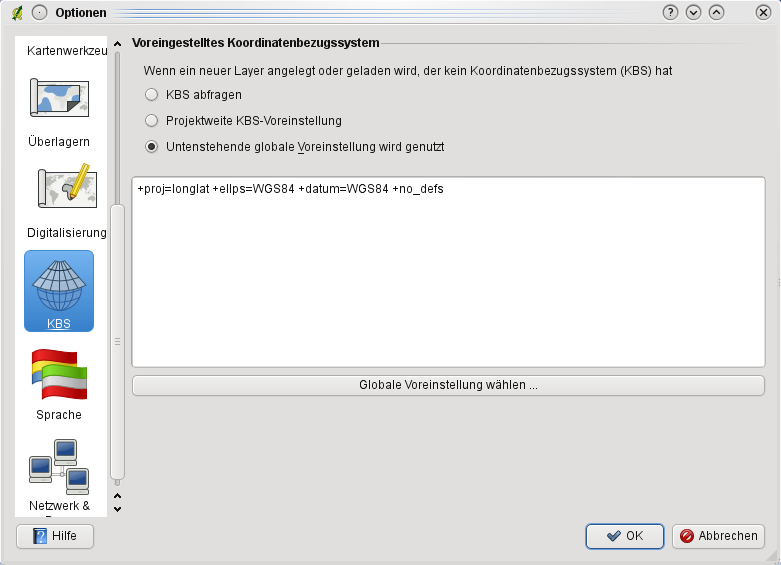
\includegraphics[clip=true, width=12cm]{crsdialog}
\end{center}
\end{figure}

% If you want to define the coordinate reference system for a certain layer
% without CRS information, you can also do that in the \tab{General} tab of the
% raster (\ref{label_generaltab}) and vector (\ref{vectorgeneraltab}) properties 
% dialog. If your layer already has a CRS defined, it
% will be displayed as shown in Figure~\ref{fig:vector_symbology}.
Si vous voulez définir le système de coordonnées de référence pour certaines couches sans information de projection, vous pouvez également faire cela dans l'onglet \tab{Général} de la boîte de dialogue propriété de la couche raster (\ref{label_generaltab}) ou vecteur (\ref{vectorgeneraltab}).  Si votre couche a déjà une projection définie, elle sera affichée comme indiqué dans la figure~\ref{fig:vector_symbology}.

% \section{Define On The Fly (OTF) Projection}\label{label_projstart}
\section{Définir une projection à la volée (OTF)}\label{label_projstart}

% \qg does not have OTF projection enabled by default, and this function is
% currently only supported for vector layers. To use OTF projection, you must
% open the \dropmenuopttwo{mActionOptions}{Project Properties} dialog, select a
% CRS and activate the \checkbox{Enable on the fly projection} checkbox.
% There are two ways to open the dialog:
Dans \qg, la projection à la volée n'est pas activée par défaut. Cette fonction est seulement gérée pour les couches vectorielles. Pour utiliser la projection à la volée, vous devez ouvrir la boîte de dialogue \dropmenuopttwo{mActionOptions}{Propriétés du projet}, sélectionner un  SCR et valider la case à cocher \checkbox{Activer la projection à la volée}. Il y a deux manières pour ouvrir la boîte de dialogue :

\begin{enumerate}
% \item Select \dropmenuopttwo{mActionOptions}{Project Properties} from the
% \mainmenuopt{Edit} (Gnome, OSX) or \mainmenuopt{Settings} (KDE, Windows) menu.
\item Sélectionnez \dropmenuopttwo{mActionOptions}{Propriétés du projet} à partir du  menu \mainmenuopt{Fichier} (Gnome, OSX) ou du menu \mainmenuopt{Préférences} (KDE, Windows).

% \item Click on the \toolbtntwo{mIconProjectionDisabled}{projector} icon in the
% lower right-hand corner of the statusbar.
\item Cliquez sur l'icône \toolbtntwo{mIconProjectionDisabled}{Statut de la projection} dans le coin en bas à droite de la barre de statut.
\end{enumerate}

% If you have already loaded a layer, and want to enable OTF projection, the
% best practice is to open the \tab{Coordinate Reference System} tab of the
% \dialog{Project Properties} dialog, select the CRS of the currently loaded
% layer, and activate the \checkbox{Enable on the fly projection} checkbox. The
% \toolbtntwo{mIconProjectionEnabled}{projector} icon will show a green hook
% and all subsequently loaded vector layers will be OTF projected to the
% defined CRS.
Si vous avez déjà chargé une couche, et désirez activer la projection à la volée, la meilleure façon de faire est d'ouvrir l'onglet \tab{Système de coordonnées de référence} de la boîte de dialogue \dialog{Propriétés du projet}, de sélectionner le SCR de la couche chargée, et d'activer la case \checkbox{Activer la projection à la volée}. L'icône \toolbtntwo{mIconProjectionEnabled}{Statut de la projection} affichera un symbole vert et toutes les couches vecteurs chargées plus tard seront projetées à la volée dans le SCR défini.
 
% The \tab{Coordinate Reference System} tab of the \dialog{Project Properties}
% dialog contains five important components as shown in Figure
% \ref{fig:projections} and described below.
L'onglet \tab{Système de Coordonnées de Référence} de la boîte de dialogue\\
\dialog{Propriétés du projet} contient cinq composants importants comme indiqué sur la figure \ref{fig:projections} et décrit ci-dessous.

\begin{figure}[ht]
   \begin{center}
%    \caption{Projection Dialog \nixcaption}\label{fig:projections}\smallskip
   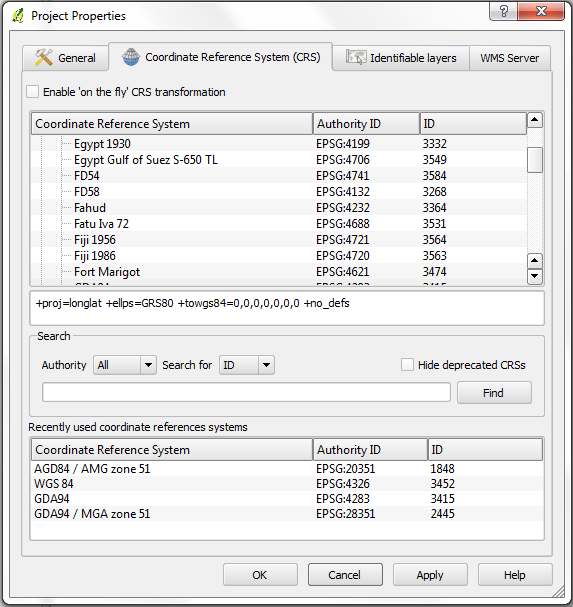
\includegraphics[clip=true, width=10cm]{projectionDialog}\caption{Boîte de dialogue Système de Coordonnées de Référence (SCR) \nixcaption} \label{fig:projections}
\end{center}
\end{figure}

\begin{enumerate}
% \item \textbf{Enable on the fly projection}\index{Projections!enabling} -
% this checkbox is used to enable or disable OTF projection. When off, each
% layer is drawn using the coordinates as read from the data source. When on,
% the coordinates in each layer are projected to the coordinate reference
% system defined for the map canvas.
\item \textbf{Activer la projection à la volée :}\index{Projections!activer}  cette case à cocher est utilisée pour activer ou désactiver la projection à la volée. Lorsqu'elle est décochée, chaque couche est dessinée en utilisant les coordonnées lues dans la source de données. Lorsqu'elle est activée, les coordonnées de chaque couche sont projetées dans le système de coordonnées de référence défini pour la carte.
% \item \textbf{Coordinate Reference System} - this is a list of all CRS
% supported by \qg, including Geographic, Projected and Custom coordinate
% reference systems. To use a CRS, select it from the list by expanding
% the appropriate node and selecting the CRS. The active CRS is preselected.
\item \textbf{Système de Coordonnées de Référence :} c'est une liste de tous les SCR gérés par \qg, incluant les systèmes de coordonnées de référence  géographiques, projetés et personnalisés. Pour utiliser un SCR, sélectionnez-le  dans la liste en déroulant le noeud approprié et en choisissant le système de coordonnées. Le SCR actif est présélectionné.
% \item \textbf{Proj4 text} - this is the CRS string used by the Proj4
% projection engine. This text is read-only and provided for informational
% purposes.
\item \textbf{Texte Proj4 :} c'est la chaîne, décrivant le SCR, qui est utilisée  par le moteur de projection Proj4. Ce texte est en lecture seule et est fourni  à titre informatif.
% \item \textbf{Search} - if you know the EPSG identifier or the name 
% for a Coordinate Reference System, you can use the search feature to find it.
% Enter the identifier and click on \button{Find}.
\item \textbf{Rechercher :} si vous connaissez le code EPSG, l'identifiant ou le nom d'un système de coordonnées de référence, vous pouvez utiliser la fonction rechercher pour le retrouver. Entrez le code et cliquez sur le bouton \button{Trouver}, cochez la case \checkbox{Masquer les SCR obsolètes} pour n'obtenir que les projections valides.
% \item \textbf{Recently used CRS} - if you have certain CRS that you frequently 
% use in your everyday GIS work, these will be displayed in the table 
% at the bottom of the Projection Dialog. Click on one of the{se buttons to select 
% the associated CRS.
\item \textbf{SCR utilisés récemment :} si vous utilisez certains SCR fréquemment dans vos travaux quotidiens, ils seront affichés dans la table en bas de la fenêtre de projection.
\end{enumerate}

\begin{Tip}
% \caption{\textsc{Project Properties Dialog}}
\caption{\textsc{Boîte de dialogue Propriétés du projet}}
% If you open the \dialog{Project Properties} dialog from the
% \mainmenuopt{Edit} (Gnome, OSX) or \mainmenuopt{Settings} 
% (KDE, Windows) menu, you must click on the \tab{Coordinate Reference
% System} tab to view the CRS settings. Opening the dialog from the
% \toolbtntwo{mIconProjectionEnabled}{projector} icon will automatically bring
% the \tab{Coordinate Reference System} tab to the front.
Si vous ouvrez la boîte de dialogue \dialog{Propriétés du projet} à partir du menu \mainmenuopt{Fichier} (Gnome, OSX) ou du menu \mainmenuopt{Préférences}  (KDE, Windows), vous devez cliquer sur l'onglet \tab{Système de Coordonnées de Référence} pour voir les définitions des SCR. Ouvrir la boîte de dialogue à partir de l'icône \toolbtntwo{mIconProjectionEnabled}{Statut de la projection} vous amènera  directement dans l'onglet \tab{Système de Coordonnées de Référence}. \end{Tip}  % \section{Custom Coordinate Reference System}\label{sec:customprojections}
% \index{Projections!custom}
\section{Système de Coordonnées de Référence personnalisé}
\label{sec:customprojections}
\index{Projections!personnalisation}

% If \qg does not provide the coordinate reference system you need, you
% can define a custom CRS. To define a CRS, select
% \dropmenuopttwo{mIconNew}{Custom CRS} from the \mainmenuopt{Edit} 
% (Gnome, OSX) or \mainmenuopt{Settings} (KDE, Windows) menu.
% Custom CRS are stored in your \qg user database. In addition to your custom
% CRS, this database also contains your spatial bookmarks and other custom data. 
Si \qg ne fournit pas le système de coordonnées de référence dont vous avez besoin, vous pouvez en définir un. Pour cela, sélectionnez \dropmenuopttwo{mIconNew}{Projection personnalisée} à partir du menu \mainmenuopt{Éditer} (Gnome, OSX) ou \mainmenuopt{Préférences} (KDE, Windows).  Les SCR personnalisés sont stockés dans votre base de données utilisateur de \qg.  En plus de ceux-ci, cette base de données contient également vos signets  spatiaux et autres données personnalisées.

\begin{figure}[ht]
   \begin{center}
%    \caption{Custom CRS Dialog \nixcaption}\label{fig:customprojections}\smallskip
   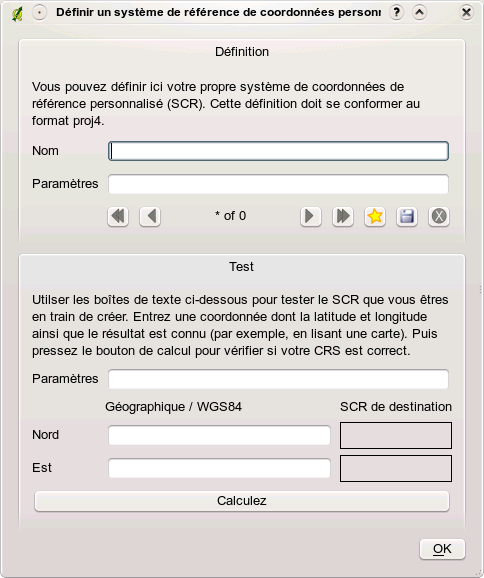
\includegraphics[clip=true, width=8cm]{customProjectionDialog}
   \caption{Boîte de dialogue SCR  personnalisé\nixcaption} \label{fig:customprojections}
\end{center}  
\end{figure}

% Defining a custom CRS in \qg requires a good understanding of the Proj.4
% projection library. To begin, refer to the Cartographic Projection Procedures
% for the UNIX Environment - A User's Manual by Gerald I. Evenden, U.S.
% Geological Survey Open-File Report 90-284, 1990 (available at \url{ftp://ftp.remotesensing.org/proj/OF90-284.pdf}).
% This manual describes the use of the \usertext{proj.4} and related command line
% utilities. The cartographic parameters used with \usertext{proj.4} are
% described in the user manual, and are the same as those used by \qg. 
Définir un SCR personnalisé dans \qg nécessite une bonne compréhension de la bibliothèque de projection Proj4. Pour commencer, référez vous aux Procédures de Projection Cartographique pour l'environnement UNIX - Un manuel d'utilisateur de Gerald I. Evenden, U.S. Geological Survey Open-File Report 90-284, 1990 (disponible sur \url{ftp://ftp.remotesensing.org/proj/OF90-284.pdf}).
Ce manuel décrit l'utilisation de \usertext{proj.4} et les applications en lignes de commandes liées. Les paramètres cartographiques utilisés avec \usertext{proj.4} sont décrit dans le manuel utilisateur et sont les mêmes que ceux utilisés par \qg.

% The \dialog{Custom Coordinate Reference System Definition} dialog requires
% only two parameters to define a user CRS: 
La boîte de dialogue \dialog{Définir un système de coordonnées de référence personnalisé} nécessite seulement deux paramètres pour définir un  SCR utilisateur :
% ==== Erreur de traduction dans le titre de la boite (GUI) :
% ==== permutation Référence et Coordonnées (incohérence avec abr SCR)
\begin{enumerate}
% \item a descriptive name and
\item un nom descriptif et
% \item the cartographic parameters in PROJ.4 format.
\item les paramètres cartographiques au format PROJ.4.
\end{enumerate}
% To create a new CRS, click the \toolbtntwo{mIconNew}{New} button and enter a
% descriptive name and the CRS parameters. After that you can save your CRS by
% clicking the button \toolbtntwo{mActionFileSave}{Save}.
Pour créer un nouveau SCR, cliquez sur le bouton \toolbtntwo{mIconNew}{Nouveau}  et entrez un nom descriptif et les paramètres du SCR. Après cela, vous pouvez  le sauvegarder en cliquant sur le bouton \toolbtntwo{mActionFileSave}{Sauvegarder}.

% Note that the \guilabel{Parameters} must begin with a \usertext{+proj=}-block,
% to represent the new coordinate reference system.
Remarquez que les \guilabel{Paramètres} doivent débuter par un  bloc \usertext{+proj=} pour représenter le nouveau système de coordonnées de référence.

% You can test your CRS parameters to see if they give sane results by
% clicking on the \button{Calculate} button inside the \guiheading{Test} block 
% and pasting your CRS parameters into
% the \guilabel{Parameters} field. Then enter known WGS 84 latitude and longitude
% values in \guilabel{North} and \guilabel{East} fields respectively. 
% Click on \button{Calculate} and compare the results with the known values in
% your coordinate reference system. 
% ========> Reprise car sinon incompréhensible
Vous pouvez tester vos paramètres de SCR pour voir s'ils produisent des  résultats valides en utilisant le bouton \button{Calculer} dans le bloc  \guiheading{Test}. Copiez vos paramètres de projection dans le champ \guilabel{Paramètres}, puis entrez des latitude et longitude connues en WGS 84 dans les champs \guilabel{Nord} et \guilabel{Est} respectivement. Cliquez sur le bouton \button{Calculer} et comparez les résultats avec les valeurs connues dans votre système de coordonnées de référence.
